\documentclass[aspectratio=169,10pt]{beamer}

\usepackage[T1]{fontenc}
\usepackage{lmodern}
\usepackage{microtype}
\usepackage{amsmath}
\usepackage{booktabs}
\usepackage{tabularx}
\usepackage{array}
\usepackage{tikz}
\usetikzlibrary{arrows.meta,positioning,calc,fit}

\definecolor{A6Blue}{RGB}{47,93,140}
\definecolor{A6Green}{RGB}{42,127,98}
\definecolor{A6Orange}{RGB}{194,122,44}
\definecolor{A6Red}{RGB}{180,76,67}
\definecolor{A6Gray}{RGB}{92,101,111}
\definecolor{A6Light}{RGB}{242,245,248}
\definecolor{A6LightBlue}{RGB}{231,238,247}
\definecolor{A6LightGreen}{RGB}{229,241,235}
\definecolor{A6LightOrange}{RGB}{249,237,221}
\definecolor{A6LightRed}{RGB}{247,231,229}

\usetheme{default}
\setbeamertemplate{navigation symbols}{}
\setbeamersize{text margin left=7mm,text margin right=7mm}
\setbeamercolor{normal text}{fg=black!84,bg=white}
\setbeamercolor{frametitle}{fg=black!88,bg=white}
\setbeamerfont{frametitle}{size=\large,series=\bfseries}
\setbeamerfont{title}{series=\bfseries,size=\LARGE}
\setbeamerfont{subtitle}{size=\large}
\setbeamercolor{structure}{fg=A6Blue}
\setbeamercolor{alerted text}{fg=A6Red}
\setbeamercolor{block title}{fg=white,bg=A6Blue}
\setbeamercolor{block body}{fg=black!84,bg=A6LightBlue}
\setbeamertemplate{itemize item}{\color{A6Blue}\small$\blacktriangleright$}
\setbeamertemplate{itemize subitem}{\color{A6Gray}\scriptsize$\bullet$}
\setbeamertemplate{footline}{%
  \leavevmode%
  \hbox{%
    \begin{beamercolorbox}[wd=\paperwidth,ht=2.6ex,dp=1.1ex,rightskip=7mm plus1fil]{date in head/foot}%
      \color{A6Gray}\scriptsize\insertframenumber/\inserttotalframenumber
    \end{beamercolorbox}%
  }%
}

\newcolumntype{Y}{>{\raggedright\arraybackslash}X}
\newcolumntype{L}[1]{>{\raggedright\arraybackslash}p{#1}}
\newcommand{\code}[1]{\texttt{#1}}
\newcommand{\good}[1]{\textcolor{A6Green}{\textbf{#1}}}
\newcommand{\bad}[1]{\textcolor{A6Red}{\textbf{#1}}}
\newcommand{\yes}{\textcolor{A6Green}{\textbf{yes}}}
\newcommand{\no}{\textcolor{A6Red}{\textbf{no}}}
\newcommand{\stagebox}[3]{%
  \begin{tikzpicture}[baseline=(n.base)]
    \node[rounded corners=2pt,draw=#1,fill=#1!10,inner xsep=4pt,inner ysep=2pt,
          text width=0.88\linewidth,align=left] (n)
      {\scriptsize\textbf{#2}\;#3};
  \end{tikzpicture}%
}

\title{Algorithm 6}
\subtitle{The Complete Internal Search Pipeline}
\author{Egyptian medicine-name search engineering review}
\date{5 August 2026}

\begin{document}

\begin{frame}[plain]
  \titlepage
  \vspace{-4mm}
  \begin{center}
    \small From raw text to ranked medicine families, confirmation, and abstention
  \end{center}
\end{frame}

\begin{frame}{What Algorithm 6 Receives and Returns}
\begin{columns}[T,onlytextwidth]
\column{0.47\textwidth}
\begin{block}{Input}
\small
A raw query string or structured unreadable-text request.
\begin{center}
\code{MYMLAX}
\quad or \quad
\code{text: RIV}\\[-1mm]
\code{unreadable\_mode: after}
\end{center}
The hidden benchmark target is never passed to search.
\end{block}

\begin{block}{Catalog}
\small
25,066 product records are grouped into \textbf{17,476 commercial-name
families}. Ranking happens at family level; package variants remain attached
for display.
\end{block}

\column{0.49\textwidth}
\begin{block}{Output}
\small
\begin{itemize}
  \item up to 20 ranked medicine families;
  \item variants, ingredients, examples, and evidence reasons;
  \item \code{ambiguous} or \code{no\_match} response status;
  \item optional likely-match label that still requires confirmation.
\end{itemize}
\end{block}

\begin{alertblock}{Safety contract}
\small
The system retrieves candidates. It never certifies a prescription or permits
automatic dispensing. Every positive result still requires user confirmation.
\end{alertblock}
\end{columns}
\end{frame}

\begin{frame}{The Entire Algorithm, Flattened}
\centering
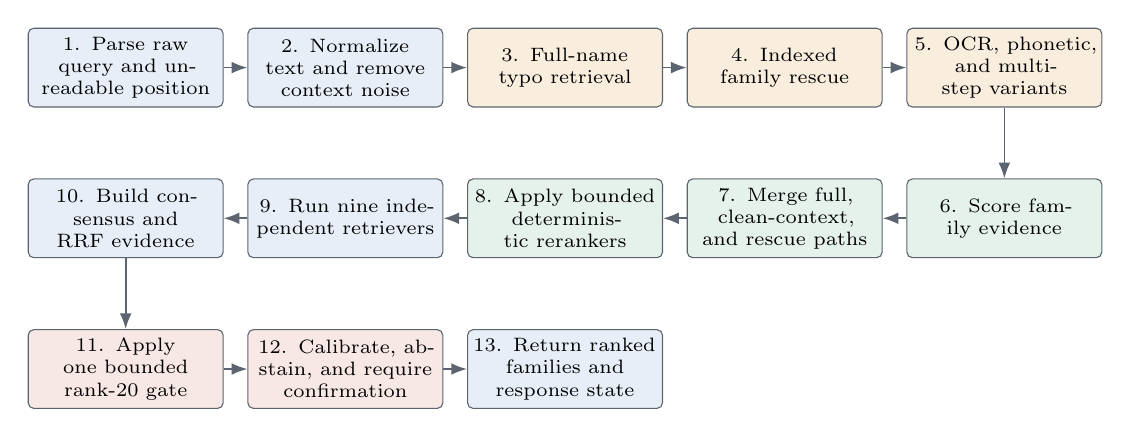
\begin{tikzpicture}[
  node distance=4mm and 3mm,
  box/.style={rounded corners=2pt,draw=A6Gray,align=center,text width=23mm,
              minimum height=10mm,font=\scriptsize,inner sep=2.5pt},
  arrow/.style={-{Latex[length=2mm]},draw=A6Gray,line width=0.6pt}
]
\node[box,fill=A6LightBlue] (q) {1. Parse raw query and unreadable position};
\node[box,fill=A6LightBlue,right=of q] (n) {2. Normalize text and remove context noise};
\node[box,fill=A6LightOrange,right=of n] (f) {3. Full-name typo retrieval};
\node[box,fill=A6LightOrange,right=of f] (r) {4. Indexed family rescue};
\node[box,fill=A6LightOrange,right=of r] (v) {5. OCR, phonetic, and multi-step variants};

\node[box,fill=A6LightGreen,below=9mm of v] (s) {6. Score family evidence};
\node[box,fill=A6LightGreen,left=of s] (m) {7. Merge full, clean-context, and rescue paths};
\node[box,fill=A6LightGreen,left=of m] (d) {8. Apply bounded deterministic rerankers};
\node[box,fill=A6LightBlue,left=of d] (p) {9. Run nine independent retrievers};
\node[box,fill=A6LightBlue,left=of p] (c) {10. Build consensus and RRF evidence};

\node[box,fill=A6LightRed,below=9mm of c] (g) {11. Apply one bounded rank-20 gate};
\node[box,fill=A6LightRed,right=of g] (a) {12. Calibrate, abstain, and require confirmation};
\node[box,fill=A6LightBlue,right=of a] (o) {13. Return ranked families and response state};

\draw[arrow] (q)--(n); \draw[arrow] (n)--(f); \draw[arrow] (f)--(r); \draw[arrow] (r)--(v);
\draw[arrow] (v)--(s); \draw[arrow] (s)--(m); \draw[arrow] (m)--(d); \draw[arrow] (d)--(p); \draw[arrow] (p)--(c);
\draw[arrow] (c)--(g); \draw[arrow] (g)--(a); \draw[arrow] (a)--(o);
\end{tikzpicture}

\vspace{3mm}
\small
The next slides open every numbered box. No predecessor algorithm is treated as
an unexplained component.
\end{frame}

\begin{frame}{Offline Catalog Preparation, With Stored Examples}
\scriptsize
Preparation runs once. The examples below are the actual forms reused at query
time, not descriptions of a hidden model.

\vspace{1mm}
\begin{tabularx}{\linewidth}{@{}L{0.18\linewidth}L{0.25\linewidth}L{0.27\linewidth}Y@{}}
\toprule
\textbf{Representation} & \textbf{Stored example} & \textbf{Lookup created} & \textbf{Query it can support} \\
\midrule
Normalized name & \code{CLEXANE} $\rightarrow$ \code{CLEXANE} & exact and token maps & \code{clexane} finds the same family \\
Compact name & \code{CLEX-A NE} $\rightarrow$ \code{CLEXANE} & punctuation-free exact key & spacing/OCR artifact \code{CLEX A NE} \\
Prefix and suffix & \code{RIVOTRIL}, reversed \code{LIRTOVIR} & prefix and reversed-prefix maps & \code{RIV} or visible ending \code{TRIL} \\
Character pieces & \code{MYOLAX} $\rightarrow$ \code{MY, YO, OL, LA, AX} & 2-, 3-, 4-gram and BM25+ matrices & \code{MYMLAX} still shares \code{MY, LA, AX} \\
Consonant shape & \code{KETOROLAC} $\rightarrow$ \code{KTRLK} & skeleton and length buckets & \code{KITORILIC} also becomes \code{KTRLK} \\
Pronunciation keys & \code{PHARMA}, \code{FARMA} $\rightarrow$ \code{PRM} & medicine key, Match Rating, NYSIIS, Soundex & \code{PH/F} sound substitution \\
Deletion forms & delete one character from each family key & delete-key map and SymSpell radius 3 & \code{LANYU} can reach \code{LANTUS} candidates \\
Family structure & \code{ABIMOL EXTRA} with head \code{ABIMOL} & family head, variants, ingredients, examples & visible head \code{ABIMOL} retrieves its longer family \\
\bottomrule
\end{tabularx}

\vspace{1mm}
\stagebox{A6Green}{Size after grouping}{25,066 product rows become 17,476
commercial-name families; package variants stay attached to the family output.}
\end{frame}

\begin{frame}{Parse the Query and the Unreadable Position}
\small
The parser accepts ordinary text and explicit information about unseen
characters. Position changes which catalog relationship counts as evidence.

\begin{table}
\centering
\begin{tabularx}{\linewidth}{@{}L{0.18\linewidth}L{0.24\linewidth}L{0.27\linewidth}Y@{}}
\toprule
\textbf{Mode} & \textbf{Input example} & \textbf{Required catalog shape} & \textbf{Interpretation} \\
\midrule
none & \code{pndol} & ordinary fuzzy match & all visible characters form the query \\
after & \code{ABIMOL [?]} & candidate starts with \code{ABIMOL} and is longer & unreadable characters follow \\
before & \code{[?] MOL} & candidate ends with \code{MOL} and is longer & unreadable characters precede \\
middle & \code{AB [?] OL} & candidate starts with \code{AB}, ends with \code{OL}, and is longer & two visible anchors surround an unreadable region \\
\bottomrule
\end{tabularx}
\end{table}

\vspace{1mm}
\begin{alertblock}{Why this is not a wildcard everywhere}
\small
The location is explicit. A prefix claim cannot silently become a suffix or
middle claim, which would multiply unrelated candidates.
\end{alertblock}
\end{frame}

\begin{frame}{Normalization, One Transformation at a Time}
\scriptsize
Normalization creates two representations because token scorers need spaces
while character scorers do not.

\begin{table}
\centering
\begin{tabularx}{\linewidth}{@{}L{0.10\linewidth}L{0.29\linewidth}L{0.29\linewidth}Y@{}}
\toprule
\textbf{Step} & \textbf{Input} & \textbf{Output} & \textbf{Reason} \\
\midrule
1 & \code{Clex-A NE 40 mg tab} & \code{CLEX-A NE 40 MG TAB} & uppercase makes case irrelevant \\
2 & \code{CLEX-A NE 40 MG TAB} & \code{CLEX A NE 40 MG TAB} & punctuation becomes one space \\
3 & repeated or edge spaces & one internal space, no edge space & token positions become stable \\
4a & normalized text & \code{CLEX A NE 40 MG TAB} & preserve tokens for WRatio and token-sort \\
4b & normalized text & \code{CLEXANE40MGTAB} & remove separators for edit, n-gram, and phonetic search \\
\bottomrule
\end{tabularx}
\end{table}

\vspace{1mm}
\stagebox{A6Green}{Second example}{\code{mymlax} $\rightarrow$
normalized \code{MYMLAX} $\rightarrow$ compact \code{MYMLAX}; no character is
corrected during normalization.}

\begin{alertblock}{Boundary}
Normalization changes representation only. It does not know that
\code{MYMLAX} should retrieve \code{MYOLAX}; retrieval handles that later.
\end{alertblock}
\end{frame}

\begin{frame}{Context Cleanup, Token by Token}
\small
The original query is always searched. A second query is created only when
recognized dosage, unit, route, or form tokens are present.

\begin{table}
\centering
\begin{tabularx}{\linewidth}{@{}L{0.28\linewidth}L{0.18\linewidth}L{0.16\linewidth}Y@{}}
\toprule
\textbf{Normalized token} & \textbf{Class} & \textbf{Action} & \textbf{Running cleaned output} \\
\midrule
\code{CLEX}, \code{A}, \code{NE} & possible name text & keep & \code{CLEX A NE} \\
\code{40} & number next to a unit & remove & \code{CLEX A NE} \\
\code{MG} & recognized unit & remove & \code{CLEX A NE} \\
\code{TAB} & recognized form & remove & \code{CLEX A NE} \\
\bottomrule
\end{tabularx}
\end{table}

\begin{columns}[T,onlytextwidth]
\column{0.48\textwidth}
\stagebox{A6Green}{Example A}{\code{CLEX-A NE 40 MG TAB}
$\rightarrow$ \code{CLEX A NE}.}
\column{0.48\textwidth}
\stagebox{A6Green}{Example B}{\code{AUGMENTIN 1 GM TAB}
$\rightarrow$ \code{AUGMENTIN}.}
\end{columns}

\vspace{2mm}
Both raw and cleaned forms are searched. If no recognized context exists, as
in \code{MYMLAX}, no second pass runs. A leading numeric brand token is kept
unless surrounding context proves it is a dose.
\end{frame}

\begin{frame}{Full-Name Typo Retrieval}
\small
The first path sends the normalized full query to the fast product-name
retriever. It returns product candidates before family rescue starts.

\begin{center}
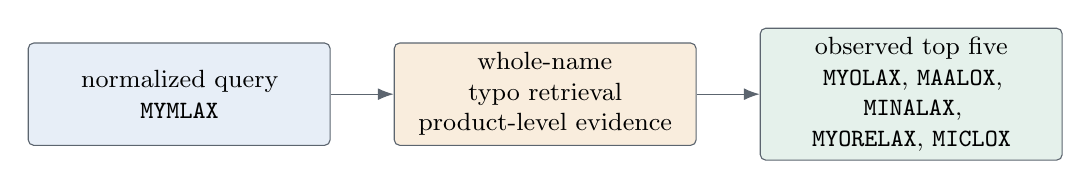
\begin{tikzpicture}[
  node distance=8mm,
  box/.style={rounded corners=2pt,draw=A6Gray,align=center,text width=36mm,
              minimum height=13mm,font=\small},
  arrow/.style={-{Latex[length=2mm]},draw=A6Gray}
]
\node[box,fill=A6LightBlue] (q) {normalized query\\\code{MYMLAX}};
\node[box,fill=A6LightOrange,right=of q] (retr) {whole-name typo retrieval\\product-level evidence};
\node[box,fill=A6LightGreen,right=of retr] (top) {observed top five\\\code{MYOLAX}, \code{MAALOX},\\\code{MINALAX}, \code{MYORELAX}, \code{MICLOX}};
\draw[arrow] (q)--(retr); \draw[arrow] (retr)--(top);
\end{tikzpicture}
\end{center}

\begin{table}
\centering
\scriptsize
\begin{tabularx}{\linewidth}{@{}L{0.17\linewidth}L{0.19\linewidth}L{0.20\linewidth}Y@{}}
\toprule
\textbf{Input} & \textbf{Full-name result} & \textbf{What succeeded} & \textbf{Why another path may still run} \\
\midrule
\code{MYMLAX} & \code{MYOLAX} rank 1 & one middle replacement & family evidence still audits the order \\
\code{CLEX-A NE 40 MG TAB} & \code{CLEXANE} rank 1 after cleaned pass & context removal exposes the brand & raw and cleaned lists are both retained \\
\code{LANS} & target family may be weak & four visible characters only & short-head and delete-key rescue add candidates \\
\bottomrule
\end{tabularx}
\end{table}
\end{frame}

\begin{frame}{Indexed Family Rescue, Lookup by Lookup}
\scriptsize
Rescue runs when the full-name list is weak or uncertain, after context
cleanup, for unreadable-position requests, and for three- or four-character queries.

\begin{tabularx}{\linewidth}{@{}L{0.20\linewidth}L{0.24\linewidth}L{0.24\linewidth}Y@{}}
\toprule
\textbf{Lookup} & \textbf{Query example} & \textbf{Catalog evidence} & \textbf{Candidate produced} \\
\midrule
Exact compact & \code{CLEX A NE} & compact key \code{CLEXANE} & family \code{CLEXANE} \\
Prefix & \code{RIV} & families beginning \code{RIV...} & \code{RIVO}, \code{RIVOTRIL}, others \\
Reversed suffix & \code{MOL} & reversed key begins \code{LOM} & \code{ABIMOL} families \\
Character grams & \code{MYMLAX} & shared \code{MY}, \code{LA}, \code{AX} & \code{MYOLAX} enters the pool \\
Consonant skeleton & \code{KITORILIC}$\rightarrow$\code{KTRLK} & \code{KETOROLAC}$\rightarrow$\code{KTRLK} & wrong-vowel candidate \\
Phonetic bucket & \code{FARMA}$\rightarrow$\code{PRM} & \code{PHARMA}$\rightarrow$\code{PRM} & sound-preserving candidate \\
Delete key & \code{LANYU} deletion forms & overlap with \code{LANTUS} deletion forms & \code{LANTUS} candidate \\
Family head & \code{ABIMOL} & validated head of \code{ABIMOL EXTRA} & longer family with variants \\
\bottomrule
\end{tabularx}

\vspace{1mm}
No lookup determines rank. Each one contributes family IDs to a union that is
scored in later stages.
\end{frame}

\begin{frame}{Bound the Rescue Candidate Pool Before Scoring}
\small
Indexed retrieval can return thousands of families for a short query. The
prefilter removes families with no plausible visible evidence.

\begin{tabularx}{\linewidth}{@{}L{0.11\linewidth}L{0.27\linewidth}L{0.28\linewidth}Y@{}}
\toprule
\textbf{Step} & \textbf{Input example} & \textbf{Test} & \textbf{Output example} \\
\midrule
1 & union for \code{LANS} & first character equal or confusable & discard unrelated initial letters \\
2 & remaining family IDs & length within the configured local window & retain \code{LANTUS}-length names \\
3 & survivors & shared grams, skeleton, phonetic, or head evidence & keep families with an explainable path \\
4 & still too many IDs & stable family-ID order & cap at 2,200 before expensive scoring \\
\bottomrule
\end{tabularx}

\vspace{2mm}
\stagebox{A6Orange}{Why the cap is safe but imperfect}{The cap controls runtime.
Removing compatible-length scanning still lowers OCR Hit@20 from 73.28\% to
71.77\%, so prefilter recall remains measurable.}
\end{frame}

\begin{frame}{Generate General OCR and Typo Variants}
\scriptsize
Variants are generated from reusable error mechanisms. They are never keyed to
a medicine name.

\begin{tabularx}{\linewidth}{@{}L{0.18\linewidth}L{0.28\linewidth}L{0.24\linewidth}Y@{}}
\toprule
\textbf{Mechanism} & \textbf{Reusable rule} & \textbf{Input $\rightarrow$ generated form} & \textbf{Candidate evidence} \\
\midrule
Keyboard/order & adjacent key, repeat, omission, adjacent swap & \code{TAVANCI}$\rightarrow$\code{TAVANIC} & transposition candidate \\
Visual digit & \code{0/O}, \code{1/I/L}, \code{2/Z}, \code{3/E}, \code{4/A}, \code{5/S}, \code{6/G}, \code{8/B} & \code{C0LCHICINE}$\rightarrow$\code{COLCHICINE} & exact transformed family key \\
Ligature & \code{RN/M}, \code{CL/D}, \code{IV/N} in both directions & \code{RNI...}$\rightarrow$\code{MI...} & merged-stroke candidate \\
Phonetic & \code{PH/F}, \code{CK/K}, \code{X/KS}, \code{QU/KW}, \code{GH/G}, \code{SH/CH} & \code{COUFSED}$\rightarrow$\code{COUGHSED} & pronunciation-preserving candidate \\
Vowel frame & replace or omit vowels, retain consonant order & \code{KITORILIC}$\rightarrow$\code{KETOROLAC} & both skeletons are \code{KTRLK} \\
Multi-step & bounded combinations of two or three rules & \code{uraranx}$\rightarrow$\code{ORAMAX} & synthetic non-regression chain \\
\bottomrule
\end{tabularx}

\vspace{2mm}
\begin{alertblock}{Guard against combinatorial explosion}
\scriptsize
Every generator has a fixed output limit and an evidence discount. A generated
form adds candidates; it does not overwrite the query or automatically become
rank 1. No table contains medicine-specific query exceptions.
\end{alertblock}
\end{frame}

\begin{frame}{Family Score: Exact Formula and One Full Calculation}
\footnotesize
For query $q$ and candidate family $f$, every evidence term is normalized to
$[0,1]$ before applying its fixed coefficient.

\begin{align*}
S(q,f)={}&1.25E + 0.58L + 0.52L_w + 0.16P + 0.10S_f\\
&+0.10G_2 + 0.18G_3 + 0.16C + 0.14H\\
&+0.10U + 0.24A + 0.16V.
\end{align*}

\begin{table}
\centering
\scriptsize
\begin{tabular}{@{}lrrrrrrrrrrrr@{}}
\toprule
\textbf{Pair} & $E$ & $L$ & $L_w$ & $P$ & $S_f$ & $G_2$ & $G_3$ & $C$ & $H$ & $U$ & $A$ & $V$ \\
\midrule
\code{MYMLAX}/\code{MYOLAX} & 0 & .833 & .833 & .333 & .500 & .429 & .143 & 1 & 1 & 0 & .833 & 1 \\
\bottomrule
\end{tabular}
\end{table}

\scriptsize
The weighted sum is about $1.75$. Same first character adds $0.12$, and equal
length with $L_w\geq0.76$ adds $0.18$, producing about $2.05$. It exceeds the
$0.62$ admission threshold. The score admits \code{MYOLAX}; later reranking
decides its position.
\end{frame}

\begin{frame}{Family Score Features, Edit and Boundary Evidence}
\scriptsize
Each row shows the exact input to one feature and the value it contributes
before weighting.

\begin{tabularx}{\linewidth}{@{}L{0.08\linewidth}L{0.23\linewidth}L{0.30\linewidth}Y@{}}
\toprule
\textbf{Term} & \textbf{Input pair} & \textbf{Calculation} & \textbf{Output and meaning} \\
\midrule
$E$ & \code{CLEXANE}/\code{CLEXANE} & compact strings equal & $1.000$, exact family \\
$L$ & \code{MYMLAX}/\code{MYOLAX} & $1-1/6$ & $0.833$, one ordinary edit \\
$L_w$ & \code{KITORILIC}/\code{KETOROLAC} & lower costs for learned vowel confusions & $0.794$ versus raw $0.667$ \\
$P$ & \code{RIV}/\code{RIVOTRIL} & 3 shared leading characters divided by 8 & $0.375$, visible prefix \\
$S_f$ & \code{MOL}/\code{ABIMOL} & 3 shared ending characters divided by 6 & $0.500$, visible suffix \\
$G_2$ & \code{MYMLAX}/\code{MYOLAX} & shared \{\code{MY,LA,AX}\}; union size 7 & $3/7=0.429$ \\
$G_3$ & same pair & only \code{LAX} shared; union size 7 & $1/7=0.143$ \\
\bottomrule
\end{tabularx}
\end{frame}

\begin{frame}{Family Score Features, Shape and Sequence Evidence}
\scriptsize
\begin{tabularx}{\linewidth}{@{}L{0.08\linewidth}L{0.23\linewidth}L{0.30\linewidth}Y@{}}
\toprule
\textbf{Term} & \textbf{Input pair} & \textbf{Transformation or calculation} & \textbf{Output and meaning} \\
\midrule
$C$ & \code{KITORILIC}/\code{KETOROLAC} & remove vowels, merge confusion groups & both become \code{KTRLK}; $C=1$ \\
$H$ & \code{PHARMA}/\code{FARMA} & \code{PH/F} and sound groups & both become \code{PRM}; $H=1$ \\
$U$ & \code{RIV}/\code{RIVOTRIL} & letters appear in order over a span of 3 & density $1$, coverage $3/8$, so $U=0.75$ \\
$A$ & \code{MYMLAX}/\code{MYOLAX} & 5 equal positions divided by maximum length 6 & $A=0.833$ \\
$V$ & \code{MYMLAX}/\code{MYOLAX} & shorter length divided by longer length & $V=6/6=1$ \\
$V$ & \code{RIV}/\code{RIVOTRIL} & $3/8$ & $0.375$, warns that most text is unseen \\
\bottomrule
\end{tabularx}

\vspace{2mm}
\stagebox{A6Orange}{Why features are combined}{\code{RIV} has perfect visible
order but only 37.5\% length coverage. Sequence evidence alone must not certify
\code{RIVOTRIL}.}
\end{frame}

\begin{frame}{Score Bonuses, Penalties, and Admission Examples}
\scriptsize
The weighted sum is adjusted only when a defined evidence pattern occurs.

\begin{tabularx}{\linewidth}{@{}L{0.19\linewidth}L{0.24\linewidth}L{0.13\linewidth}Y@{}}
\toprule
\textbf{Rule} & \textbf{Concrete pair} & \textbf{Adjustment} & \textbf{Why} \\
\midrule
same first character & \code{MYMLAX}/\code{MYOLAX} & $+0.12$ & both start \code{M} \\
confusable first character & \code{K...}/\code{C...} & $+0.06$ & \code{C/K/Q} share a configured confusion group \\
near-equal length + strong weighted edit & \code{MYMLAX}/\code{MYOLAX} & $+0.18$ & equal length and $L_w=.833$ \\
strong prefix + edit & a long candidate with most of its prefix visible & $+0.08$ & two signals agree \\
strong edit + position & one mild OCR substitution & $+0.22$ & $L_w\geq.84$ and $A\geq.70$ \\
weak partial prefix & \code{RIV}/\code{RIVOTRIL} & at least $-0.18$ & candidate is much longer than visible text \\
short query + weak edit & \code{H}/\code{RIVO} & $-0.22$ & one character cannot identify a family \\
weak edit and weak sound/shape & unrelated family & $-0.20$ & no independent support \\
weak prefix, grams, and edit & unrelated family & $-0.10$ & all lexical channels are weak \\
\bottomrule
\end{tabularx}

\vspace{1mm}
Keep score $\geq0.62$. A positional OCR exception can pass at $0.58$ only when
the first character, positional score, and visible-length coverage also pass.
\end{frame}

\begin{frame}{Score Family Heads Without Collapsing Unrelated Drugs}
\small
A package can contain a stable brand head plus a variant suffix. Head scoring
lets visible brand text retrieve the family, but grouping requires validated
catalog structure.

\begin{center}
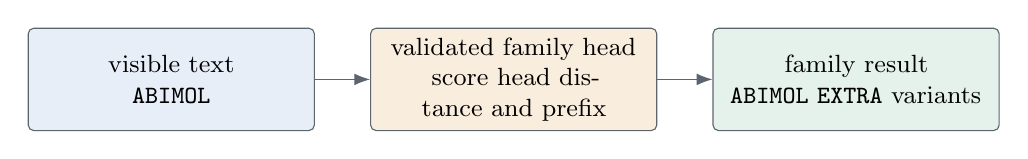
\begin{tikzpicture}[
  node distance=7mm,
  box/.style={rounded corners=2pt,draw=A6Gray,align=center,text width=34mm,
              minimum height=13mm,font=\small},
  arrow/.style={-{Latex[length=2mm]},draw=A6Gray}
]
\node[box,fill=A6LightBlue] (q) {visible text\\\code{ABIMOL}};
\node[box,fill=A6LightOrange,right=of q] (head) {validated family head\\score head distance and prefix};
\node[box,fill=A6LightGreen,right=of head] (fam) {family result\\\code{ABIMOL EXTRA} variants};
\draw[arrow] (q)--(head); \draw[arrow] (head)--(fam);
\end{tikzpicture}
\end{center}

\begin{table}
\centering
\scriptsize
\begin{tabularx}{\linewidth}{@{}L{0.18\linewidth}L{0.25\linewidth}L{0.19\linewidth}Y@{}}
\toprule
\textbf{Visible query} & \textbf{Catalog structure} & \textbf{Action} & \textbf{Reason} \\
\midrule
\code{ABIMOL} & validated head of \code{ABIMOL EXTRA} & score the head and return the family & user may see only the stable brand head \\
\code{LANS} & short head evidence for \code{LANTUS} & admit as a candidate, not certainty & removal loses \code{LANS}$\rightarrow$\code{LANTUS} from top 20 \\
\code{ABC} & several unrelated \code{ABC ...} families & keep separate candidates & a shared token is not proof of one variant family \\
\bottomrule
\end{tabularx}
\end{table}
\end{frame}

\begin{frame}{Merge Three Deterministic Evidence Paths}
\scriptsize
Candidates are merged by compact family key, not by product row.

\begin{center}
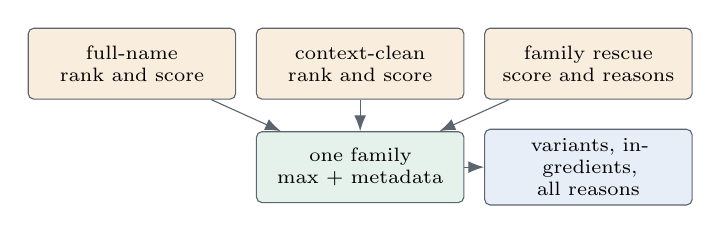
\begin{tikzpicture}[
  node distance=2.5mm,
  box/.style={rounded corners=2pt,draw=A6Gray,align=center,text width=24mm,
              minimum height=9mm,font=\scriptsize},
  arrow/.style={-{Latex[length=2mm]},draw=A6Gray}
]
\node[box,fill=A6LightOrange] (full) {full-name\\rank and score};
\node[box,fill=A6LightOrange,right=of full] (ctx) {context-clean\\rank and score};
\node[box,fill=A6LightOrange,right=of ctx] (res) {family rescue\\score and reasons};
\node[box,fill=A6LightGreen,below=4mm of ctx] (merge) {one family\\max + metadata};
\node[box,fill=A6LightBlue,right=of merge] (out) {variants, ingredients,\\all reasons};
\draw[arrow] (full)--(merge); \draw[arrow] (ctx)--(merge); \draw[arrow] (res)--(merge); \draw[arrow] (merge)--(out);
\end{tikzpicture}
\end{center}

\begin{table}
\centering
\scriptsize
\begin{tabularx}{\linewidth}{@{}L{0.14\linewidth}L{0.38\linewidth}L{0.22\linewidth}Y@{}}
\toprule
\textbf{Query} & \textbf{Evidence before merge} & \textbf{Merge operation} & \textbf{Final family record} \\
\midrule
\code{MYMLAX} & full path: \code{MYOLAX} rank 1; rescue: edit and n-gram evidence; no clean pass & group by compact key; keep maximum score and every reason & one \code{MYOLAX} record; agreement bonus $+0.08$ \\
\code{CLEX...40 MG TAB} & full path: noisy list; clean path: \code{CLEXANE} rank 1; rescue: exact compact family & group by compact key; attach product variants to the family & one \code{CLEXANE} record; full/clean bonus $+0.06$ \\
\bottomrule
\end{tabularx}
\end{table}
\end{frame}

\begin{frame}{Deterministic Reranking Uses Bounded Corrections}
\scriptsize
The default order is score descending, clarification state, then stable name.
Edit distance is never used as one global tie-break rule.

\begin{tabularx}{\linewidth}{@{}L{0.20\linewidth}L{0.30\linewidth}L{0.22\linewidth}Y@{}}
\toprule
\textbf{Correction class} & \textbf{Evidence required} & \textbf{Concrete example} & \textbf{Bound} \\
\midrule
Unique nearest & decisive raw or weighted distance advantage & \code{MYOLANA}$\rightarrow$\code{MYOLAX} & equal-distance ties do not force a move \\
Exact visual/ligature & transformed key exactly reaches a family & \code{C0LCHICINE}$\rightarrow$\code{COLCHICINE} & distance and score limits must also pass \\
Phonetic + position & sound key and same-position characters agree & \code{ECOFIXIM}$\rightarrow$\code{CEFIXIME} & phonetic key alone cannot promote \\
Skeleton + position & consonant frame and visible positions agree & \code{KITORILIC}$\rightarrow$\code{KETOROLAC} & wrong-vowel evidence needs anchors \\
Family head & validated head plus compatible family & \code{LANYU}$\rightarrow$\code{LANTUS} & unrelated prefixes stay separate \\
Multi-step exact chain & bounded chain reaches an exact family key & \code{uraranx}$\rightarrow$\code{ORAMAX} & restore prior top if advantage is weak \\
\bottomrule
\end{tabularx}

\vspace{2mm}
\begin{alertblock}{Rank-1 protection}
\scriptsize
Fallback and generated candidates cannot change the first result without a
unique, rule-specific advantage. This guard matters empirically: removing all
deterministic reranking lowers OCR Hit@1 from 50.43\% to 40.52\%.
\end{alertblock}
\end{frame}

\begin{frame}{Independent Retrievers, Each With an Observed Example}
\scriptsize
After the deterministic family list is ready, nine independent lists search the
same 17,476 families. Each returns at most 20 names.

\begin{tabularx}{\linewidth}{@{}L{0.20\linewidth}L{0.31\linewidth}L{0.29\linewidth}Y@{}}
\toprule
\textbf{Retriever} & \textbf{Input $\rightarrow$ representation} & \textbf{Observed output} & \textbf{What the vote means} \\
\midrule
Jaro--Winkler & compact \code{TEFA} against compact families & \code{TELFAST} source rank 1 & order and common prefix agree \\
Match Rating & \code{ABASCOLOGY} $\rightarrow$ compressed pronunciation code & \code{ABASAGLAR} rank 1 & consonant pronunciation agrees \\
RapidFuzz WRatio & normalized \code{LACTULOSE}; direct and partial ratios & \code{LACTO} rank 3 & candidate is a strong partial form \\
NYSIIS & \code{MYOLOGY} $\rightarrow$ pronunciation-oriented code & \code{MYOLAX} rank 1 & an independent sound encoding agrees \\
BM25+ 3-grams & \code{LACTULOSE}$\rightarrow$ overlapping three-character pieces & \code{LACTO} rank 12 & informative local pieces survive \\
\bottomrule
\end{tabularx}
\end{frame}

\begin{frame}{Remaining Independent Retrievers, With Examples}
\scriptsize
\begin{tabularx}{\linewidth}{@{}L{0.20\linewidth}L{0.31\linewidth}L{0.29\linewidth}Y@{}}
\toprule
\textbf{Retriever} & \textbf{Input $\rightarrow$ representation} & \textbf{Observed output} & \textbf{What the vote means} \\
\midrule
SymSpell & compact \code{OSFOCU}; symmetric deletes to distance 3 & \code{OSTOCAL} rank 1 & bounded edit candidate exists \\
RapidFuzz token-sort & normalize and sort tokens before ratio & \code{TELFAST} rank 2 for \code{TEFA} & token/string view supplies a second vote \\
Soundex & \code{TELBACE} $\rightarrow$ coarse sound code & \code{TELFAST} rank 1 & broad phonetic backstop agrees \\
Dice 2-grams & \code{TEFA}$\rightarrow$\{\code{TE,EF,FA}\} & \code{TELFAST} rank 15 & shared \code{TE} and \code{FA} supply a third vote \\
\bottomrule
\end{tabularx}

\vspace{3mm}
The deterministic family list is source 10. These nine methods run in parallel;
none filters the next one. One source can be wrong without deleting candidates
from the other lists.
\end{frame}

\begin{frame}{Build One Consensus Record per Family}
\scriptsize
All ten top-20 lists are merged by compact family key. A candidate stores every
source rank and four query-to-family similarities.

\begin{columns}[T,onlytextwidth]
\column{0.45\textwidth}
\begin{block}{Stored features}
\begin{itemize}
  \item source count $C$;
  \item reciprocal-rank fusion score;
  \item Levenshtein similarity;
  \item Jaro--Winkler similarity;
  \item character-bigram Dice;
  \item learned OCR-confusion similarity, diagnostic only.
\end{itemize}
\end{block}

\column{0.52\textwidth}
\begin{block}{Reciprocal-rank fusion}
\[
\operatorname{RRF}(f)=
\sum_{s\in\mathcal{S}_f}\frac{1}{60+r_{s,f}}
\]
$r_{s,f}$ is the rank in source $s$. Rank 1 contributes $1/61=0.01639$;
rank 14 contributes $1/74=0.01351$. The constant 60 makes several independent
votes matter more than one exceptional rank.
\end{block}
\end{columns}

\vspace{1mm}
\begin{tabularx}{\linewidth}{@{}L{0.19\linewidth}L{0.16\linewidth}L{0.16\linewidth}L{0.16\linewidth}L{0.15\linewidth}Y@{}}
\toprule
\textbf{Real record} & \textbf{Sources} & \textbf{RRF} & \textbf{Lev.} & \textbf{Jaro} & \textbf{Dice} \\
\midrule
\code{MYMLAX}$\rightarrow$\code{MYOLAX} & 9 of 10 & .1439 & .8333 & .9111 & .600 \\
\bottomrule
\end{tabularx}
The nine source ranks are 1, 14, 1, 1, 2, 1, 1, 3, and 1. Learned-confusion
similarity is 0.86 and remains diagnostic in the current rank-20 policy.
\end{frame}

\begin{frame}{Consensus Ordering Is Explicit and Deterministic}
\small
The candidate union is sorted lexicographically by this tuple:
\[
\left(
-C,\ -\operatorname{RRF},\ -L,\ -J,\ \text{name},\ \text{family key}
\right).
\]

\begin{enumerate}
  \item More independent sources wins first.
  \item Better rank positions across those sources win next.
  \item Levenshtein and Jaro--Winkler resolve remaining evidence ties.
  \item Name and family key make the output stable across runs.
\end{enumerate}

\begin{table}
\centering
\scriptsize
\begin{tabular}{@{}lrrrrl@{}}
\toprule
\textbf{Query \code{MYMLAX}} & \textbf{sources} & \textbf{RRF} & \textbf{Lev.} & \textbf{Jaro} & \textbf{Order reason} \\
\midrule
\code{MYOLAX} & 9 & .143876 & .833 & .911 & more sources \\
\code{MYORELAX} & 7 & .109917 & .625 & .856 & remains below \\
\bottomrule
\end{tabular}
\end{table}

\begin{alertblock}{What this order does not do}
The consensus order does not replace the deterministic first result. A tested broad
rank-1 consensus rule gained 27 synthetic cases and lost 138, so it remains
disabled. Consensus is used only as a bounded retrieval rescue.
\end{alertblock}
\end{frame}

\begin{frame}{The Only Enabled Consensus Rewrite: One Rank-20 Slot}
\small
The deterministic order is copied first. At most one outside consensus candidate
may replace the final slot.

\begin{center}
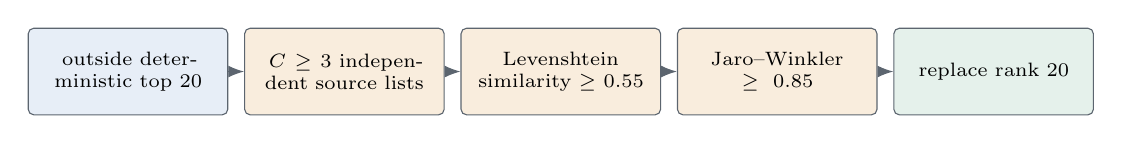
\begin{tikzpicture}[
  node distance=2mm,
  box/.style={rounded corners=2pt,draw=A6Gray,align=center,text width=23mm,
              minimum height=11mm,font=\scriptsize},
  arrow/.style={-{Latex[length=2mm]},draw=A6Gray}
]
\node[box,fill=A6LightBlue] (outside) {outside deterministic top 20};
\node[box,fill=A6LightOrange,right=of outside] (votes) {$C\geq3$ independent source lists};
\node[box,fill=A6LightOrange,right=of votes] (lev) {Levenshtein similarity $\geq0.55$};
\node[box,fill=A6LightOrange,right=of lev] (jaro) {Jaro--Winkler $\geq0.85$};
\node[box,fill=A6LightGreen,right=of jaro] (insert) {replace rank 20};
\draw[arrow] (outside)--(votes); \draw[arrow] (votes)--(lev); \draw[arrow] (lev)--(jaro); \draw[arrow] (jaro)--(insert);
\end{tikzpicture}
\end{center}

\begin{table}
\centering
\scriptsize
\begin{tabular}{@{}lrrrrl@{}}
\toprule
\textbf{Input $\rightarrow$ candidate} & \textbf{sources} & \textbf{Lev.} & \textbf{Jaro} & \textbf{Pass?} & \textbf{Result} \\
\midrule
\code{TEFA}$\rightarrow$\code{TELFAST} & 3 & .571 & .886 & \yes & inserted at rank 20 \\
\code{OSCAR}$\rightarrow$\code{OSTOCAL} & 2 & .571 & .832 & \no & source and Jaro gates fail \\
\code{NEUROTROPHIC}$\rightarrow$\code{NEUROCET} & 4 & .417 & .850 & \no & Levenshtein gate fails \\
\code{RIV}$\rightarrow$\code{RIVOTRIL} & 2 & .375 & .854 & \no & source and Levenshtein fail \\
\bottomrule
\end{tabular}
\end{table}

The first 19 families remain unchanged. This gate adds 2 OCR Hit@20 cases with
0 paired losses and changes no synthetic top-$k$ result. The broader rank-1
gate is disabled in the policy file.
\end{frame}

\begin{frame}{Worked Example: \code{TEFA} to \code{TELFAST}}
\scriptsize
This row shows why Algorithm 6 needs independent candidate sources.

\begin{tabularx}{\linewidth}{@{}L{0.22\linewidth}Y@{}}
\toprule
\textbf{Step} & \textbf{Observed execution} \\
\midrule
1. Parse and compact & \code{TEFA} stays \code{TEFA}; no context or unreadable marker. \\
2. Deterministic retrieval & \code{TELFAST} is outside the top 20; top 1 is \code{TERA}. \\
3. Independent lists & Jaro--Winkler rank 1, token-sort rank 2, Dice bigrams rank 15. \\
4. Source agreement & $C=3$, exactly the minimum required. \\
5. Lexical gates & Levenshtein $=1-3/7=0.571$; Jaro--Winkler $=0.886$. Both pass. \\
6. Bounded rewrite & \code{TELFAST} replaces rank 20. Ranks 1--19 remain unchanged. \\
7. Final output & top 1 \code{TERA}; \code{TELFAST} at rank 20; status \code{ambiguous}. \\
\bottomrule
\end{tabularx}

\vspace{2mm}
\begin{center}
\stagebox{A6Green}{Result}{Hit@20 changes from failure to success without
claiming that \code{TELFAST} is certainly the intended medicine.}
\end{center}
\end{frame}

\begin{frame}{Worked Example: \code{MYMLAX} to \code{MYOLAX}}
\small
This row succeeds before the external slot, then consensus measures how strong
the agreement is.

\begin{columns}[T,onlytextwidth]
\column{0.48\textwidth}
\begin{block}{Character evidence}
\begin{itemize}
  \item one replacement, \code{M}$\rightarrow$\code{O};
  \item Levenshtein similarity $=5/6=0.833$;
  \item Jaro--Winkler $=0.911$;
  \item same length and strong positional agreement.
\end{itemize}
\end{block}

\column{0.49\textwidth}
\begin{block}{Source evidence}
\code{MYOLAX} occurs in 9 of 10 lists: deterministic, BM25+, Dice, Jaro,
Match Rating, NYSIIS, token-sort, WRatio, and SymSpell.
\end{block}

\begin{exampleblock}{Final output}
\code{MYOLAX} remains rank 1. No external slot is needed. Current policy returns
\code{ambiguous}, \code{needs\_clarification=true}, and probability $0.0$
because the optional abstention model is not enabled.
\end{exampleblock}
\end{columns}
\end{frame}

\begin{frame}{Final Safety State and the Disabled Optional Calibrator}
\scriptsize
The code can calculate a calibrated correctness probability when the policy
contains an \code{abstention} block. The current policy contains no such block,
so calibration returns probability 0 and never changes the message.

\begin{tabularx}{\linewidth}{@{}L{0.24\linewidth}Y@{}}
\toprule
\textbf{Calibration inputs} & \textbf{Exact contents} \\
\midrule
Top-family evidence & source count, RRF, Levenshtein, Jaro--Winkler, bigram Dice \\
Top-1 versus top-2 gaps & source-count, RRF, Levenshtein, and Jaro differences \\
Response context & candidate count, query length, rank-1 promotion flag, external-slot flag \\
Optional model & standardized logistic regression over these values; never changes ranking \\
Current policy & no \code{abstention} configuration; probability $0.0$ and likely-match flag \code{false} \\
\bottomrule
\end{tabularx}

\vspace{2mm}
\begin{columns}[T,onlytextwidth]
\column{0.48\textwidth}
\begin{block}{Candidates exist}
Status \code{ambiguous}; message asks the user to compare evidence and confirm
the medicine. Every result keeps \code{needs\_clarification=true}.
\end{block}
\column{0.49\textwidth}
\begin{alertblock}{No candidate survives}
Status \code{no\_match}; example \code{H}$\rightarrow$ no result. One visible
character is not converted into a forced medicine family.
\end{alertblock}
\end{columns}

\vspace{1mm}
An experimental 0.63 calibrator was measured separately on provisional
audit-clean subsets, but it is not present in the active policy and is not a
clinical guarantee.
\end{frame}

\begin{frame}{How Every Score in the Next Slides Was Produced}
\small
No value below is copied from a paper's dataset. Every method was rerun locally
against the same two frozen evaluation sets.

\begin{tabularx}{\linewidth}{@{}L{0.23\linewidth}L{0.20\linewidth}L{0.23\linewidth}Y@{}}
\toprule
\textbf{Evaluation set} & \textbf{Cases} & \textbf{One case means} & \textbf{Metric example} \\
\midrule
OCR primary fair unique & 464 & one distinct scored compact query-target pair; real-drug collisions excluded & \code{MYMLAX}$\rightarrow$\code{MYOLAX}; rank 1 gives H@1=1 \\
Synthetic clean core & 66,257 & one fair generated corruption-target pair after collision filtering & generated typo with its catalog family target \\
\bottomrule
\end{tabularx}

\vspace{2mm}
\begin{block}{Exact score source}
\scriptsize
\code{benchmark\_04\_experiments/results/07\_algorithm\_6/}
\code{all\_evaluated\_method\_scores.csv}. The method descriptions and URLs
come from \code{results/06\_competitor\_benchmark/competitor\_inventory.csv}.
\end{block}

\stagebox{A6Orange}{Interpretation}{The GitHub or paper project supplies method
provenance. The percentages are our Egyptian medicine benchmark results, not
claims copied from those projects.}
\end{frame}

\begin{frame}{Algorithms 1 to 6 on the Same Frozen Cases}
\scriptsize
\begin{tabular}{@{}lrrrrrrr@{}}
\toprule
& \multicolumn{3}{c}{\textbf{OCR 464}} & \multicolumn{3}{c}{\textbf{Synthetic 66,257}} & \\
\cmidrule(lr){2-4}\cmidrule(lr){5-7}
\textbf{Method} & \textbf{H@1} & \textbf{H@5} & \textbf{H@20} & \textbf{H@1} & \textbf{H@5} & \textbf{H@20} & \textbf{OCR ms} \\
\midrule
Algorithm 1 & 23.71 & 31.47 & 38.15 & 83.86 & 89.72 & 92.23 & 1.28 \\
Algorithm 2 & 25.86 & 43.75 & 51.29 & 92.41 & 96.33 & 96.88 & 4.75 \\
Algorithm 3 & 25.65 & 40.95 & 53.02 & 91.84 & 96.18 & 97.12 & 6.84 \\
Algorithm 4 & 47.63 & 61.85 & 71.12 & 97.19 & 99.24 & 99.52 & 14.89 \\
Algorithm 5 & \textbf{50.43} & \textbf{63.58} & 72.84 & \textbf{98.19} & \textbf{99.65} & \textbf{99.9985} & 28.54 \\
Algorithm 6 & \textbf{50.43} & \textbf{63.58} & \textbf{73.28} & \textbf{98.19} & \textbf{99.65} & \textbf{99.9985} & 48.50 \\
\bottomrule
\end{tabular}

\vspace{2mm}
\begin{tabularx}{\linewidth}{@{}L{0.15\linewidth}Y@{}}
\toprule
\textbf{Code source} & \textbf{Local implementation} \\
\midrule
A1, A2, A3 & \code{app/app.js}; \code{external\_algorithms/english\_search\_algorithm\_fast.py}; \code{master\_commercial\_name\_search.py} \\
A4, A5, A6 & \code{algorithm\_4\_commercial\_name\_search.py}; \code{algorithm\_5\_commercial\_name\_search.py}; \code{algorithm\_6\_consensus\_search.py} \\
\bottomrule
\end{tabularx}

Algorithm 6 adds two OCR top-20 recoveries over Algorithm 5 and changes no
rank-1 result. Its additional retrievers increase mean OCR latency by 19.96 ms.
\end{frame}

\begin{frame}{External Lexical Baselines, Locally Rerun}
\scriptsize
\begin{tabular}{@{}lrrrrl@{}}
\toprule
& \multicolumn{2}{c}{\textbf{OCR 464}} & \multicolumn{2}{c}{\textbf{Synthetic 66,257}} & \\
\cmidrule(lr){2-3}\cmidrule(lr){4-5}
\textbf{Method} & \textbf{H@1} & \textbf{H@20} & \textbf{H@1} & \textbf{H@20} & \textbf{Method source} \\
\midrule
SymSpell, distance 3 & 38.58 & 55.82 & 94.22 & 98.80 & SymSpell \\
Damerau--Levenshtein & 34.27 & 59.27 & 94.78 & 99.64 & RapidFuzz \\
Exhaustive Levenshtein & 34.27 & 59.27 & 94.05 & 99.44 & RapidFuzz \\
Jaro--Winkler & 32.11 & 67.46 & 89.57 & 98.43 & Jellyfish \\
BM25+ character 3-grams & 20.26 & 47.41 & 78.19 & 92.17 & rank\_bm25 \\
Character 3-gram TF--IDF & 18.32 & 47.41 & 75.21 & 91.66 & scispaCy reference \\
RapidFuzz weighted ratio & 11.21 & 56.25 & 55.73 & 97.20 & RapidFuzz \\
Exact or prefix & 2.59 & 3.02 & 3.00 & 3.01 & local baseline \\
\bottomrule
\end{tabular}

\vspace{2mm}
\stagebox{A6Green}{Observed pattern}{Jaro--Winkler has the strongest external
OCR H@20 at 67.46\%, while Damerau--Levenshtein is stronger on synthetic H@20.
Algorithm 6 exceeds both on OCR because it combines family, character, sound,
and safety evidence.}
\end{frame}

\begin{frame}{Biomedical, Hybrid, and Phonetic Baselines}
\scriptsize
\begin{tabular}{@{}lrrrrl@{}}
\toprule
& \multicolumn{2}{c}{\textbf{OCR 464}} & \multicolumn{2}{c}{\textbf{Synthetic 66,257}} & \\
\cmidrule(lr){2-3}\cmidrule(lr){4-5}
\textbf{Method} & \textbf{H@1} & \textbf{H@20} & \textbf{H@1} & \textbf{H@20} & \textbf{Method source} \\
\midrule
BioSyn-style, sparse weight .50 & 20.47 & 53.02 & 78.17 & 93.78 & BioSyn \\
xMEN-style SapBERT + TF--IDF RRF & 16.81 & 52.37 & 48.85 & 92.30 & xMEN \\
SapBERT dense HNSW & 11.42 & 38.58 & 27.67 & 56.45 & SapBERT \\
Egyptian medicine phonetic baseline & 6.90 & 23.28 & 69.66 & 92.07 & local implementation \\
\bottomrule
\end{tabular}

\vspace{3mm}
\begin{block}{Why these scores are included}
Dense biomedical normalization methods test semantic representation; sparse
hybrids add character evidence; the phonetic baseline tests sound alone. Their
low OCR H@1 shows that prescription corruption cannot be solved by semantic or
phonetic similarity without family-aware lexical evidence.
\end{block}
\end{frame}

\begin{frame}{External Method Provenance}
\scriptsize
\begin{tabularx}{\linewidth}{@{}L{0.26\linewidth}Y@{}}
\toprule
\textbf{Methods used locally} & \textbf{Original project or implementation reference} \\
\midrule
Levenshtein, Damerau, WRatio & \href{https://github.com/rapidfuzz/RapidFuzz}{github.com/rapidfuzz/RapidFuzz} \\
Jaro--Winkler and phonetic encoders & \href{https://github.com/jamesturk/jellyfish}{github.com/jamesturk/jellyfish} \\
SymSpell & \href{https://github.com/wolfgarbe/SymSpell}{github.com/wolfgarbe/SymSpell} \\
BM25 family & \href{https://github.com/dorianbrown/rank_bm25}{github.com/dorianbrown/rank\_bm25} \\
BioSyn-style hybrid & \href{https://github.com/dmis-lab/BioSyn}{github.com/dmis-lab/BioSyn} \\
SapBERT dense retrieval & \href{https://github.com/cambridgeltl/sapbert}{github.com/cambridgeltl/sapbert} \\
xMEN-style dense+sparse RRF & \href{https://github.com/hpi-dhc/xmen}{github.com/hpi-dhc/xmen} \\
Character TF--IDF reference & \href{https://github.com/allenai/scispacy}{github.com/allenai/scispacy} \\
Phonetic method reference & \href{https://github.com/microsoft/PhoneticMatching}{github.com/microsoft/PhoneticMatching} \\
\bottomrule
\end{tabularx}

\vspace{2mm}
All adapters, catalog preparation, ranking, and scoring were executed by
\code{run\_competitor\_benchmark.py}. Source links identify the method family;
they do not imply that upstream authors evaluated this Egyptian catalog.
\end{frame}

\begin{frame}{Ablation Contract and Top-Level Paths}
\scriptsize
Reference is complete Algorithm 6 on the same 464 OCR pairs: H@1 50.431\%,
H@20 73.276\%. Each row removes only the named component, reruns the changed
pipeline, then leaves all other retrieval and consensus stages active.

\begin{tabularx}{\linewidth}{@{}L{0.20\linewidth}rrrrY@{}}
\toprule
\textbf{Removed component} & \textbf{H@1} & \textbf{$\Delta$H@1} & \textbf{H@20} & \textbf{$\Delta$H@20} & \textbf{Observed example} \\
\midrule
Nothing & \textbf{50.431} & 0 & \textbf{73.276} & 0 & \code{MYMLAX}$\rightarrow$\code{MYOLAX} rank 1 \\
Family rescue & 36.638 & $-13.793$ & 56.034 & $-17.241$ & \code{TUTORIALAE}$\rightarrow$\code{KETOROLAC}: 7 to $>20$ \\
External full-name retriever & 49.784 & $-0.647$ & 72.414 & $-0.862$ & \code{ABDUSONG LAR}$\rightarrow$\code{ABASAGLAR}: 1 to $>20$ \\
Context-clean second pass & 50.431 & 0 & 73.276 & 0 & no top-$k$ change on these 464 pairs; \code{CLEX...40 MG TAB} still explains the path \\
\bottomrule
\end{tabularx}

\vspace{2mm}
\stagebox{A6Red}{Largest dependency}{The family-rescue path is responsible for
most measured recall. Ablation effects overlap and therefore cannot be added.}
\end{frame}

\begin{frame}{Retrieval Ablations With Measured OCR Losses}
\scriptsize
\begin{tabularx}{\linewidth}{@{}L{0.22\linewidth}rrrY@{}}
\toprule
\textbf{Retrieval removed} & \textbf{H@1} & \textbf{H@20} & \textbf{$\Delta$H@20} & \textbf{Changed input $\rightarrow$ target} \\
\midrule
Short-edge retrieval & 49.784 & 70.259 & $-3.017$ & \code{RICOHIL}$\rightarrow$\code{RIVOTRIL}: 3 to $>20$ \\
Family-head rescue & 48.060 & 70.905 & $-2.371$ & \code{LANYU}$\rightarrow$\code{LANTUS}: 2 to $>20$ \\
Delete-key retrieval & 48.276 & 71.121 & $-2.155$ & \code{LANYU}$\rightarrow$\code{LANTUS}: 2 to $>20$ \\
Compatible-length scan & 49.784 & 71.767 & $-1.509$ & \code{INDULGENCE}$\rightarrow$\code{INDERAL}: 10 to $>20$ \\
Short visible-head rescue & 50.431 & 73.060 & $-0.216$ & \code{LANS}$\rightarrow$\code{LANTUS}: 20 to $>20$ \\
Short-frame rescue & 50.431 & 73.276 & $0.000$ & one H@20 gain and one loss cancel; \code{LAE}$\rightarrow$\code{LACTO} is lost \\
\bottomrule
\end{tabularx}

H@20 after removal is the complete rerun score, not a standalone component
accuracy. Shared cases explain why family-head and delete-key effects overlap.
\end{frame}

\begin{frame}{Retrieval Ablations With Zero Net OCR Top-$k$ Change}
\scriptsize
Every row below produces H@1 50.431\% and H@20 73.276\% after removal on the
464 OCR pairs.

\begin{tabularx}{\linewidth}{@{}L{0.25\linewidth}L{0.24\linewidth}Y@{}}
\toprule
\textbf{Retrieval removed} & \textbf{Example mechanism} & \textbf{What zero means} \\
\midrule
All multi-step chains & \code{uraranx}$\rightarrow$\code{ORAMAX} & other OCR sources cover this sample; synthetic H@1 loses 343 and gains 3 \\
Bounded-nearest fallback & unique nearest candidate & no OCR top-$k$ pair changed \\
Evidence-query variants & alternate evidence form & no OCR top-$k$ pair changed \\
First-character expansion & confusable \code{C/K/Q} initial & no OCR top-$k$ pair changed \\
Keyboard rescue & adjacent key or repeat & no OCR top-$k$ pair changed \\
Ligature rescue & \code{RN/M}, \code{CL/D}, \code{IV/N} & no OCR top-$k$ pair changed \\
Short-query rescue & three- or four-character pool & no net change beyond overlapping paths \\
Transposition rescue & \code{TAVANCI}$\rightarrow$\code{TAVANIC} & no OCR top-$k$ pair changed \\
Visual-deletion chains & digit/letter plus omission & no OCR top-$k$ pair changed \\
Visual-phonetic chains & visual plus sound rewrite & no OCR top-$k$ pair changed \\
\bottomrule
\end{tabularx}

Zero is sample-specific redundancy, not proof that the mechanism is useless.
\end{frame}

\begin{frame}{Scoring-Signal Ablations, Largest Effects}
\scriptsize
\begin{tabularx}{\linewidth}{@{}L{0.21\linewidth}rrrrY@{}}
\toprule
\textbf{Signal removed} & \textbf{H@1} & \textbf{$\Delta$H@1} & \textbf{H@20} & \textbf{$\Delta$H@20} & \textbf{Observed loss example} \\
\midrule
Weighted edit similarity & 49.569 & $-0.862$ & 66.164 & $-7.112$ & \code{TUTORIALAE}$\rightarrow$\code{KETOROLAC}: 7 to $>20$ \\
Raw edit similarity & 49.353 & $-1.078$ & 67.888 & $-5.388$ & same case loses uniform edit support \\
Length coverage & 50.216 & $-0.216$ & 70.259 & $-3.017$ & 15 H@20 losses, 1 gain \\
Positional evidence & 48.922 & $-1.509$ & 71.336 & $-1.940$ & \code{TEFAXATE}$\rightarrow$\code{TELFAST}: 16 to $>20$ \\
Prefix evidence & 48.707 & $-1.724$ & 71.336 & $-1.940$ & \code{RIVITAM}$\rightarrow$\code{RIVOTRIL}: 17 to $>20$ \\
Character n-grams & 48.060 & $-2.371$ & 71.983 & $-1.293$ & local pieces around corruptions disappear \\
\bottomrule
\end{tabularx}

Weighted and raw edit signals affect many of the same rows. Their deltas are
paired ablations, not independent contributions to add together.
\end{frame}

\begin{frame}{Scoring-Signal Ablations, Smaller or Rank-Only Effects}
\scriptsize
\begin{tabularx}{\linewidth}{@{}L{0.21\linewidth}rrrrY@{}}
\toprule
\textbf{Signal removed} & \textbf{H@1} & \textbf{$\Delta$H@1} & \textbf{H@20} & \textbf{$\Delta$H@20} & \textbf{Observed effect} \\
\midrule
Weighted confusion costs & 48.707 & $-1.724$ & 72.845 & $-0.431$ & \code{KETOMAN}$\rightarrow$\code{KATOMOR}: 14 to $>20$ \\
Consonant skeleton & 49.784 & $-0.647$ & 73.060 & $-0.216$ & one top-20 loss \\
Subsequence evidence & 50.000 & $-0.431$ & 73.060 & $-0.216$ & two losses and one gain \\
Phonetic evidence & 49.569 & $-0.862$ & 73.276 & 0 & \code{ECOFIXIM}$\rightarrow$\code{CEFIXIME}: rank 1 to 2 \\
Retriever agreement & 50.216 & $-0.216$ & 73.276 & 0 & \code{OSSETIA}$\rightarrow$\code{OSSICA}: rank 1 to 3 \\
Suffix evidence & 49.569 & $-0.862$ & 73.276 & 0 & \code{RIVOFLURAL}$\rightarrow$\code{RIVOTRIL}: rank 1 to 2 \\
\bottomrule
\end{tabularx}

Signals with zero H@20 delta can still protect rank 1. H@1 and H@20 answer
different questions and must both be reported.
\end{frame}

\begin{frame}{Reranker Ablations}
\scriptsize
\begin{tabularx}{\linewidth}{@{}L{0.24\linewidth}rrrY@{}}
\toprule
\textbf{Reranker removed} & \textbf{H@1} & \textbf{H@20} & \textbf{$\Delta$H@1} & \textbf{Observed effect} \\
\midrule
All deterministic reranking & 40.517 & 70.690 & $-9.914$ & \code{LANYU}$\rightarrow$\code{LANTUS}: 2 to $>20$ \\
Candidate-pool/head rerankers & 48.276 & 71.336 & $-2.155$ & 10 H@1 and 9 H@20 losses \\
Character-evidence rerankers & 48.922 & 73.276 & $-1.509$ & \code{RIVOFN2}$\rightarrow$\code{RIVOTRIL}: rank 1 to 2 \\
Strict full-name correction & 49.569 & 73.276 & $-0.862$ & \code{MYOLANA}$\rightarrow$\code{MYOLAX}: rank 1 to 2 \\
Exact-key rerankers & 50.431 & 73.276 & 0 & no top-$k$ change on OCR 464 \\
Multi-step-chain rerankers & 50.431 & 73.276 & 0 & no top-$k$ change on OCR 464 \\
Nearest-candidate rerankers & 50.431 & 73.276 & 0 & no top-$k$ change on OCR 464 \\
Weighted-edge rerankers & 50.431 & 73.276 & 0 & no top-$k$ change on OCR 464 \\
\bottomrule
\end{tabularx}

The large all-reranking drop includes overlapping correction families. It does
not imply that every zero-delta subgroup can be deleted without a fresh test.
\end{frame}

\begin{frame}{Score-Tuning, Safety, and Atomic-Flag Ablations}
\scriptsize
\begin{tabularx}{\linewidth}{@{}L{0.25\linewidth}rrY@{}}
\toprule
\textbf{Removed item} & \textbf{H@1} & \textbf{H@20} & \textbf{Interpretation} \\
\midrule
Exact-chain score augmentation & 50.431 & 73.276 & no OCR top-$k$ pair changed \\
In-place chain score tuning & 50.431 & 73.276 & no OCR top-$k$ pair changed \\
Safety clarification gate & 50.431 & 73.276 & retrieval is unchanged; top-$k$ cannot measure response safety \\
Strict full-name evidence guard flag off & 50.647 & 73.276 & 2 H@1 gains and 1 loss, so net score hides a regression \\
Strict full-name rerank flag off & 49.569 & 73.276 & 4 H@1 losses \\
Other 52 atomic flags, one at a time & 50.431 & 73.276 & no OCR top-$k$ change individually \\
\bottomrule
\end{tabularx}

The 54 atomic rows test implementation switches inside the semantic components.
The complete auditable list remains in \code{algorithm\_6\_replay\_metrics.csv}.
\end{frame}

\begin{frame}{Algorithm 6 Consensus-Source Ablations}
\scriptsize
\begin{tabularx}{\linewidth}{@{}L{0.26\linewidth}rrrY@{}}
\toprule
\textbf{Removed item} & \textbf{H@1} & \textbf{H@20} & \textbf{$\Delta$H@20} & \textbf{Observed consequence} \\
\midrule
Bounded rank-20 slot & 50.431 & 72.845 & $-0.431$ & \code{TEFA} and \code{LACTULOSE} leave top 20 \\
Jaro--Winkler source & 50.431 & 73.060 & $-0.216$ & \code{TEFA}$\rightarrow$\code{TELFAST} loses one vote \\
RapidFuzz token-sort source & 50.431 & 73.060 & $-0.216$ & same \code{TEFA} case loses one vote \\
Dice bigram source & 50.431 & 73.060 & $-0.216$ & shared \code{TE} and \code{FA} vote disappears \\
BM25+ trigram source & 50.431 & 73.060 & $-0.216$ & competing outsider replaces \code{LACTO} \\
Match Rating source & 50.431 & 73.276 & 0 & remaining sources preserve both accepted gains \\
WRatio source & 50.431 & 73.276 & 0 & remaining sources preserve both accepted gains \\
NYSIIS source & 50.431 & 73.276 & 0 & remaining sources preserve both accepted gains \\
SymSpell source & 50.431 & 73.276 & 0 & remaining sources preserve both accepted gains \\
Soundex source & 50.431 & 73.276 & 0 & remaining sources preserve both accepted gains \\
\bottomrule
\end{tabularx}

Single-source zero deltas show redundancy on this sample. They do not prove
the source never contributes candidate evidence on unseen reviewed crops.
\end{frame}

\begin{frame}{Failure Examples: Missing or Insufficient Evidence}
\scriptsize
The supplied family is outside all final top-20 lists in these rows.

\begin{tabularx}{\linewidth}{@{}L{0.14\linewidth}L{0.14\linewidth}L{0.14\linewidth}L{0.24\linewidth}Y@{}}
\toprule
\textbf{Input} & \textbf{Supplied target} & \textbf{Top 1} & \textbf{Target evidence} & \textbf{What the failure means} \\
\midrule
\code{H} & \code{RIVO} & none & 0 sources; one character & insufficient evidence; no-match is safer \\
\code{HOAVACH} & \code{AMIKACIN} & \code{HYABAK} & 0 sources; distance 6 & severe mixed corruption; retrieval, not reranking, fails \\
\code{LANSOPRAZOLE} & \code{LANTUS} & \code{PANTOPRAZOLE} & 1 source; Lev. 33.3\%; Jaro 81.1\% & supplied target is much farther than visible alternatives \\
\code{RIV} & \code{RIVOTRIL} & \code{RIVO} & 2 sources; Lev. 37.5\%; Jaro 85.4\% & exact short family and several prefixes compete \\
\code{ABACAVIR} & \code{ABASAGLAR} & \code{TECAVIR} & 1 Soundex source; Lev. 31.6\% & one phonetic vote cannot justify insertion \\
\bottomrule
\end{tabularx}

\vspace{2mm}
\stagebox{A6Orange}{Aggregate}{Of 124 top-20 misses, 97 targets appear in none
of the ten source lists. They cannot be repaired by changing the final sorter.}
\end{frame}

\begin{frame}{Failure Examples: Gate Rejection or Label Conflict}
\scriptsize
\begin{tabularx}{\linewidth}{@{}L{0.14\linewidth}L{0.14\linewidth}L{0.14\linewidth}L{0.24\linewidth}Y@{}}
\toprule
\textbf{Input} & \textbf{Supplied target} & \textbf{Top 1} & \textbf{Target evidence} & \textbf{What the failure means} \\
\midrule
\code{OSCAR} & \code{OSTOCAL} & \code{ASCOR} & 2 sources; Lev. 57.1\%; Jaro 83.2\% & Levenshtein passes; source count and Jaro fail \\
\code{NEUROTROPHIC} & \code{NEUROCET} & \code{NEUROTOP} & 4 sources; Lev. 41.7\%; Jaro 85.0\% & only Levenshtein blocks four weak votes \\
\code{LANLTA} & \code{LANTUS} & \code{LANETAL} & 2 sources; Lev. 33.3\%; Jaro 80.6\% & target is weak and returned family is one edit closer \\
\code{TOCILIZUMAB} & \code{TOCO} & \code{ALIZOLAM} & 1 WRatio source; Lev. 27.3\%; Jaro 67.4\% & target discards most visible characters; audit the label \\
\code{CINNARIZIN} & \code{MYOLAX} & \code{CINNARIZINE} & 0 sources; target distance 9; nearest 1 & visible text strongly suggests a different catalog drug \\
\bottomrule
\end{tabularx}

\vspace{2mm}
\stagebox{A6Red}{Do not tune blindly}{Twenty-seven misses have some source
support but fail a gate. Many also conflict with a closer catalog name, so crop
review must precede threshold reduction.}
\end{frame}

\begin{frame}{Runtime and Query-Time Work}
\footnotesize
\begin{tabularx}{\linewidth}{@{}L{0.23\linewidth}L{0.27\linewidth}Y@{}}
\toprule
\textbf{Part} & \textbf{Bounded work} & \textbf{Practical cost} \\
\midrule
Catalog preparation & build deterministic maps, sparse 2/3-gram matrices, phonetic arrays, and SymSpell dictionary & once per process for 17,476 families \\
Deterministic retrieval & indexed lookup plus bounded family scoring and correction rules & measured primary path mean: 28.54 ms/query \\
Independent retrieval & several catalog scans, two sparse matrix products, and SymSpell lookup & adds most Algorithm 6 overhead \\
Consensus merge & at most $10\times20=200$ source appearances; merge by family and sort & small relative to retrieval \\
Complete Algorithm 6 & all stages, gates, and output formatting & measured OCR mean: 48.50 ms/query \\
\bottomrule
\end{tabularx}

\vspace{1mm}
\begin{block}{Optimization target}
\scriptsize
Cache catalog preparation and parallelize independent source queries while
requiring exact top-20 parity. Removing evidence merely to reduce latency can
erase the two measured consensus gains.
\end{block}
\end{frame}

\begin{frame}{Executable Algorithm Summary}
\footnotesize
\begin{enumerate}
  \item Parse visible text and any before/middle/after unreadable marker.
  \item Normalize the query; optionally create a context-clean second query.
  \item Search the full catalog, then retrieve family candidates from exact,
        prefix, suffix, n-gram, skeleton, phonetic, delete, head, and length indexes.
  \item Generate bounded keyboard, visual, ligature, phonetic, vowel, and
        multi-step variants.
  \item Score candidates with raw and weighted edit, edges, n-grams, sound,
        consonants, subsequence, position, and length evidence.
  \item Merge evidence by commercial family; apply bounded deterministic
        corrections and preserve weak cases as ambiguous.
  \item Run Jaro--Winkler, Match Rating, WRatio, NYSIIS, BM25+ trigrams,
        SymSpell, token-sort, Soundex, and Dice bigrams.
  \item Merge ten lists, compute source count and RRF, and allow one external
        rank-20 candidate only after the $3/0.55/0.85$ gate.
  \item Estimate likely correctness without changing ranking; require
        confirmation or abstain.
  \item Return up to 20 family-level candidates with evidence and safety state.
\end{enumerate}

\vspace{2mm}
\begin{center}
\good{The algorithm is a controlled evidence pipeline, not one distance formula
and not one opaque earlier algorithm.}
\end{center}
\end{frame}

\begin{frame}[plain]
\centering
\vfill
{\LARGE\bfseries Algorithm 6, in one sentence}

\vspace{8mm}
\begin{minipage}{0.82\linewidth}
\centering
\large
Generate medicine-family candidates from several independent representations,
rank them with bounded character and structural evidence, add only one
consensus-supported retrieval rescue, and never convert lexical agreement into
unconfirmed clinical certainty.
\end{minipage}

\vfill
\small
Implementation: \code{benchmark\_01\_legacy/master\_algorithms/algorithm\_6\_consensus\_search.py}
\end{frame}

\end{document}
